\documentclass{article}

% URLs and hyperlinks ---------------------------------------
\usepackage{hyperref}
\hypersetup{
	colorlinks=true,
	linkcolor=blue,
	filecolor=magenta,      
	urlcolor=blue,
}
\usepackage{xurl}
%---------------------------------------------------

\usepackage{graphicx}
\usepackage{rotating}
\usepackage{mathtools}
\usepackage{enumitem}
\usepackage{gensymb}

\usepackage{xepersian}
\settextfont{Yas}
\setdigitfont{Yas}

\title{
	گزارش کار آزمایش چهارم \\
}
\author{
	گروه: \\
	اریسا احسانی \\
	سید حسین حسینی \\
	مهدی حق‌وردی \\ \\
	شعبه شش
}
\date{}
\renewcommand{\arraystretch}{1.4}

\begin{document}
	\maketitle
	\tableofcontents
	\clearpage
	
	\section{با توجه به مدار زیر،‌ جدول را تکمیل کنید}
		\begin{center}
			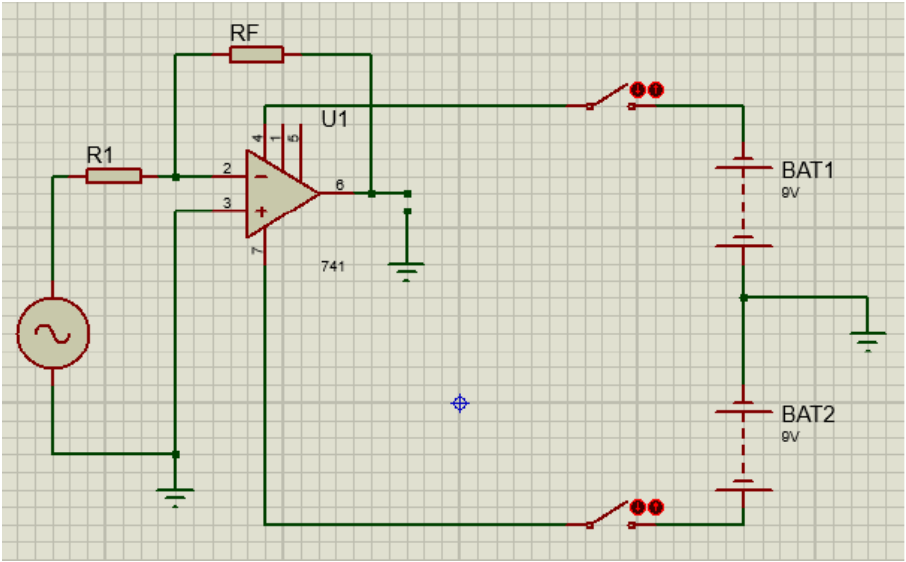
\includegraphics[width=13cm, height=8cm]{./images/4.1}
		\end{center}
		
		\begin{table}[h]
			\begin{center}
				\begin{tabular}{|c|c|c|c|c|c|}
					\hline
					\lr{Phase} & \lr{Gain} & \lr{Input} & \lr{Output} & \lr{$R_1$} & \lr{$R_f$} \\
					\hline
					\hline
					$180\degree$ & $-2.54$ & $100 \, mV$ & $256 \, mV$ & $2200$ & $5600$ \\
					\hline
					$180\degree$ & $-1$ & $100 \, mV$ & $100 \, mV$ & $5600$ & $5600$ \\
					\hline
					$180\degree$ & $-0.16$ & $100 \, mV$ & $16 \, mV$ & $33000$ & $5600$ \\
					\hline
				\end{tabular}	
			\end{center}
		\end{table}
	
	\clearpage
	\section{یک مدار غیر معکوس کننده ببندید و جدول زیر را کامل کنید}
		\begin{center}
			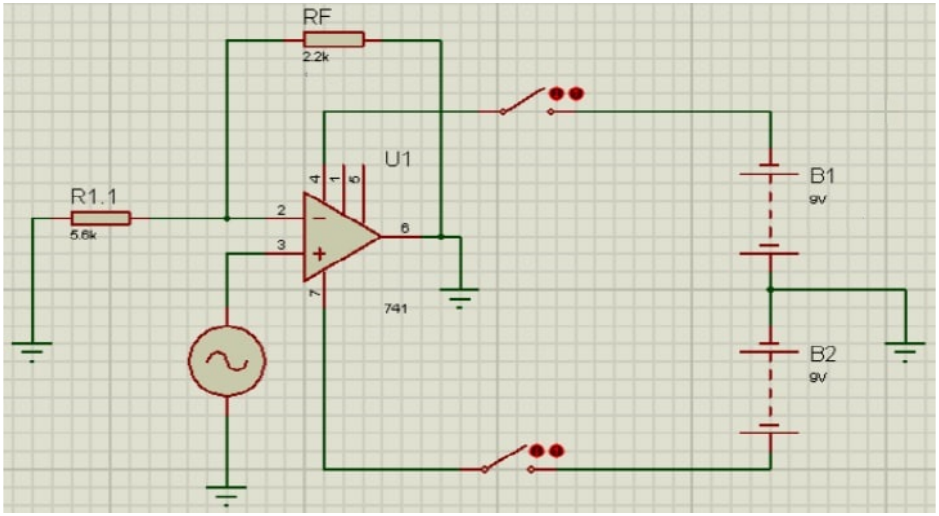
\includegraphics[width=13cm, height=8cm]{./images/4.2}	
        \end{center}
    	\begin{table}[h]
    		\begin{center}
    			\begin{tabular}{|c|c|c|c|c|c|}
    				\hline
    				\lr{Phase} & \lr{Gain} & \lr{Input} & \lr{Output} & \lr{$R_1$} & \lr{$R_f$} \\
    				\hline
    				\hline
    				$0\degree$ & $3.54$ & $100 \, mV$ & $354 \, mV$ & $2200$ & $5600$ \\
    				\hline
    				$0\degree$ & $2$ & $100 \, mV$ & $200 \, mV$ & $5600$ & $5600$ \\
    				\hline
    				$0\degree$ & $1.16$ & $100 \, mV$ & $116 \, mV$ & $33000$ & $5600$ \\
    				\hline
    			\end{tabular}	
    		\end{center}
    	\end{table}
    
	\clearpage
	\section{مداری طراحی کنید که معادله‌ی روبه‌رو را پیاده‌سازی کند}
		\begin{equation*}
			V_0 = 2V_1 - 3V_2
		\end{equation*}
	
		\begin{center}
			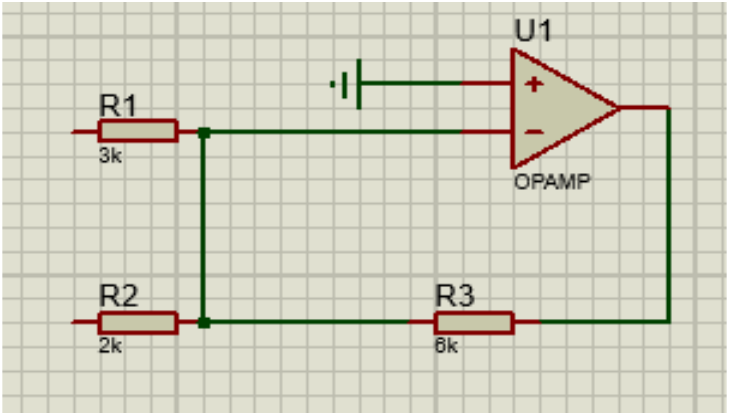
\includegraphics[width=13cm, height=8cm]{./images/4.3}	
        \end{center}
		
		\begin{table}[h]
			\begin{center}
				\begin{tabular}{|c|c|c|}
					\hline
					$V_0$ & $V_2$ & $V_1$ \\
					\hline
					\hline
					0 & 2 & 3\\
					\hline
					-1 & 1 & 1 \\
					\hline
					5 & 1 & 4\\
					\hline
				\end{tabular}
			\end{center}
		\end{table}
	\clearpage
	\section{مداری طراحی کنید که معادله‌ی روبه‌رو را پیاده‌سازی کند}
		\begin{equation*}
			V_0 = 4V_1 + 5V_2
		\end{equation*}
	
  		\begin{center}
			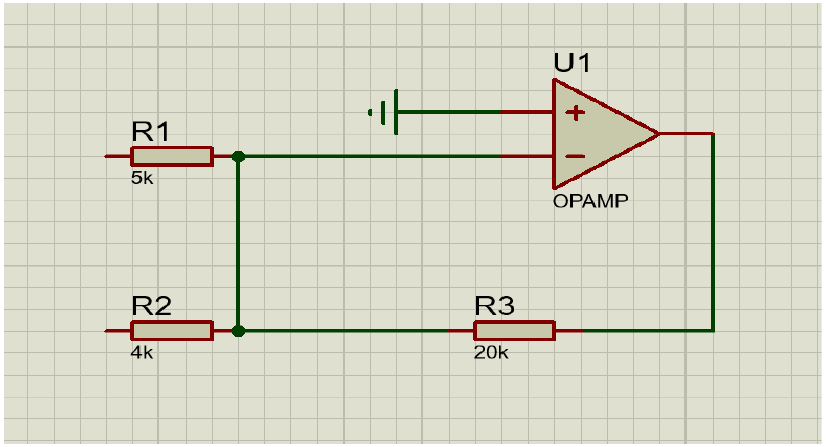
\includegraphics[width=13cm, height=8cm]{./images/4.4}    	
        \end{center}
		\begin{table}[h]
			\begin{center}
				\begin{tabular}{|c|c|c|}
					\hline
					$V_0$ & $V_2$ & $V_1$ \\
					\hline
					\hline
					9 & 1 & 1 \\
					\hline
					14 & 2 & 1 \\
					\hline
					23 & 3 & 2\\
					\hline
				\end{tabular}
			\end{center}
		\end{table}
		       	
\end{document}